% Условная компиляция для самостоятельной работы
\ifdefined\mainfile
    % Если это часть основного файла, не добавляем начало и конец документа
\else
    \documentclass[12pt, a4paper]{report}
    \usepackage{/Users/vladbelousov/Desktop/Semestr_4-FP-NSU/Настройка/library}
    \usepackage[utf8]{inputenc} % Подключение поддержки UTF-8
    \begin{document}
\fi

%%-------------------------------%%
\[ f: \mathbb{D} \to  \mathbb{R}     , \text{ } \mathbb{D} \subset \mathbb{R} ^2  , \text{ } \mathbb{D} \text{ - непустое открытое множество} \] 

Зависимость от параметра: 

\[ \begin{aligned}
    \begin{cases}
        y ' = f(t, y , \mu^* ) \\
        y(t_0 )= y_0
        \end{cases}
        \quad  \Rightarrow \quad 
        y(t, \mu^* ) \text{ - решение } 
\end{aligned} \] 

\[ \begin{aligned}
    \begin{cases}
        y ' = f(t , y , \mu ) \\
        y(t_0 )= y_0
        \end{cases} 
        \quad \Rightarrow \quad      
        y(t, \mu )  \text{ - решение } 
\end{aligned}\]

\begin{center}
    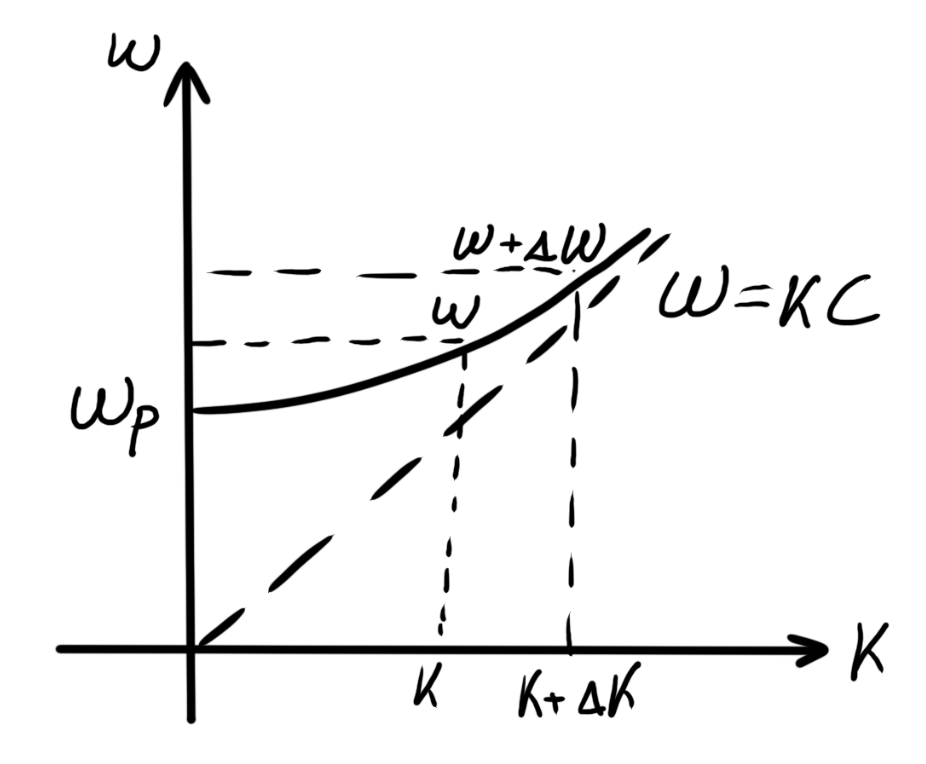
\includegraphics[width=0.4\textwidth]{/Users/vladbelousov/Desktop/Semestr_4-FP-NSU/ДфУ/Лекции_по_дням/image/26.png}
\end{center}

Пример 2: 

\[ \begin{aligned}
    \begin{cases}
        y = \mu^{* }  y ^2 = 0 \cdot y ^2 \\
        y(0 ) = 1
        \end{cases} 
        \quad \Rightarrow \quad 
        y(t,0 ) =1
\end{aligned}\] 

\[ \begin{aligned}
    \begin{cases}
        y = \mu  y ^2 = 0 \cdot y ^2 \\
        y(0 ) = 1
        \end{cases} 
        \quad \Rightarrow \quad 
        y(t,\mu ) = \frac{1}{1 - \mu t } 
\end{aligned}\] 

\begin{center}
    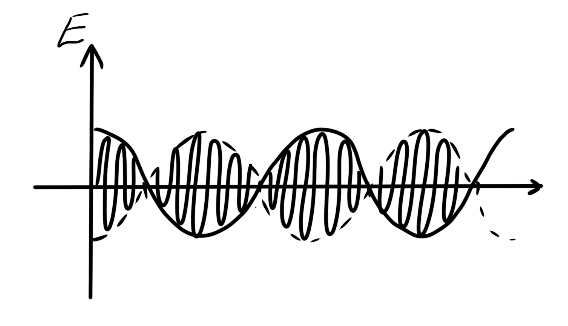
\includegraphics[width=0.5\textwidth]{/Users/vladbelousov/Desktop/Semestr_4-FP-NSU/ДфУ/Лекции_по_дням/image/27.png}
\end{center}

\begin{flushleft}
    \textbf{Теорема 2.} \textit{ \( f : B \to  \mathbb{R} , \text{ }  B \subset \mathbb{R} ^3 , \text{ } B  \) - непустое множество. Пусть  \( f \in  C(B ) \) \( \displaystyle  , \text{ } \exists  \frac{ \partial  f }{\partial  y } \in  C (B ) , \text{ }  (t_0, y_0 , \mu^* ) \in  B  \). Пусть \( y (t,\mu^* ) \) определено на  интервале \( (\alpha, \omega) \). Возьмем \( [t_1, t_2 ] \in  (\alpha , \omega) \)   }:  
    
    1) \( \exists  \Delta > 0 , \text{ }  \forall  \mu : |\mu - \mu^*   | < \Delta \Rightarrow y ( t, \mu ) \textit{ определено на } [t_1,t_2 ]  \) 

    2) \(  y(t,\mu ) \xrightarrow{\mu \to  \mu^* } y(t, \mu^*)   \text{ } \forall  t \in  [t_1,t_2 ]\) 
\end{flushleft}

Пример 2: 

\[ f(t, y ,\mu ) = \mu y ^2 , \text{ }  B = \mathbb{R} ^3 , \text{ }  f \in  C ( \mathbb{R} ^3 ) , \text{  } \exists  \frac{\partial  f }{\partial  y } \in  C (\mathbb{R} ^3 ) , \text{ }  ( 0,1,0 ) \in \mathbb{R} ^3   \] 

\[ y(t, \mu ^ * ) = y ( t, 0 ) = 1 , \text{ }  (\alpha , \omega ) = ( - \infty  , \infty ) \] 

Возьмем \( [-T, T ] \subset ( - \infty  , \infty  ) \) 

\begin{center}
    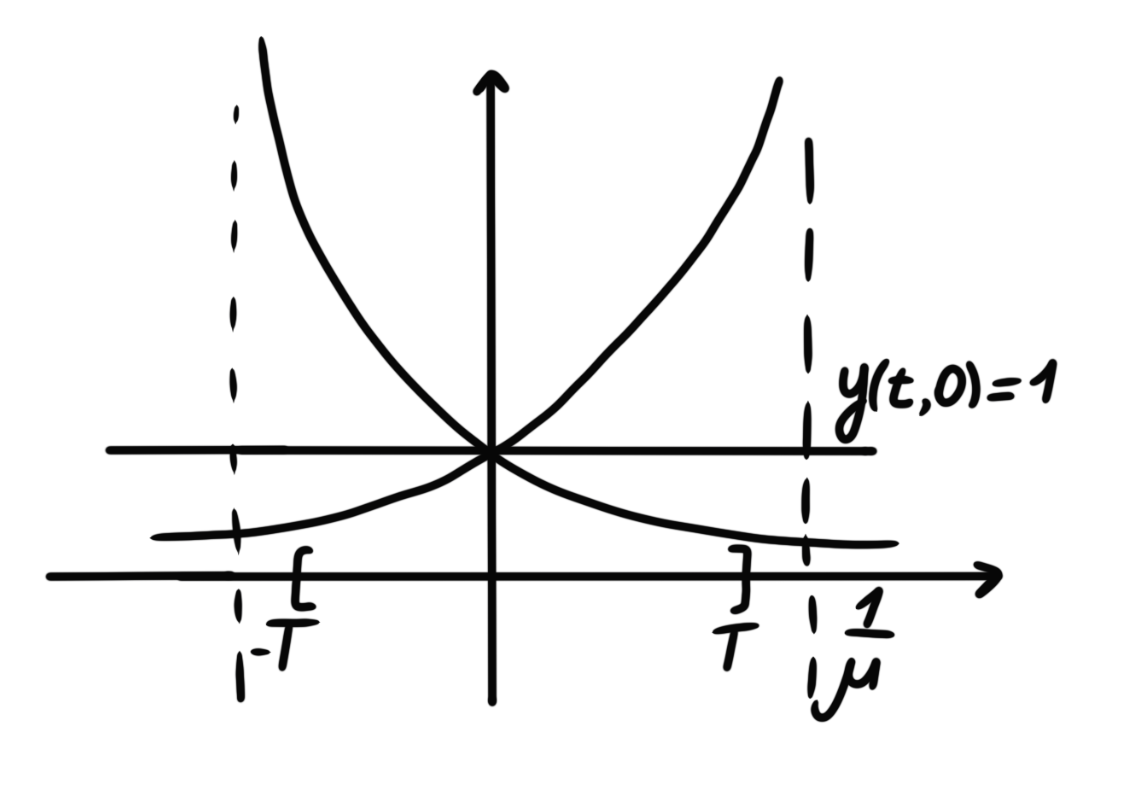
\includegraphics[width=0.5\textwidth]{/Users/vladbelousov/Desktop/Semestr_4-FP-NSU/ДфУ/Лекции_по_дням/image/28.png}
\end{center}

\[1) \text{ }  \mu > 0 : \frac{1}{\mu } > T \Leftrightarrow  \mu < \frac{1}{T  }  \quad  \mu < 0 : \frac{1}{\mu } < -T \Leftrightarrow \mu>  - \frac{1}{T }       \] 

\[ - \frac{1}{T }  < \mu < \frac{1}{ T }  \Leftrightarrow  |\mu     | < \frac{1}{T   } = \Delta   \] 

\[ 2) \text{ }  t \in [- T , T ] : \frac{1}{1 - \mu T } \xrightarrow{ \mu \to  0 } 1     \] 

\begin{proof}[Доказательство теоремы 1 с использованием теоремы 2]

    \[  \] 
    \[ \begin{aligned}
    \begin{cases}
    y ' = f(t ,y ) \\
    y (t_0 ) = y_0^ * 
    \end{cases}
    \quad  \Rightarrow \quad  y (t, y_0 ^*)
    \end{aligned} \] 
    
    \[ \begin{aligned}
        \begin{cases}
        y ' = f(t ,y ) \\
        y (t_0 ) = y_0
        \end{cases}
        \quad  \Rightarrow \quad  y (t, y_0)
        \end{aligned} \] 

        Замена переменных \( z(t, y_0 ) = y (t, t_0 ) - y_0 \) 

        \[ \begin{aligned}
        \begin{cases}
            y_t ' = z_y ' + (y_0  ' )_t  = z_t ' = f(t,y ) = f(t,z+ y_0) \\  
            z(t_0 ) = y(t_0  ) - y_0(t_0 ) = y_0 - y_0 = 0
        \end{cases}
        \end{aligned} \] 

        \[ \begin{aligned}
        \begin{cases}
            z_t ' = f(t , z+ y_0 ) \\ 
            z(t_0 )= 0 
        \end{cases}
        \text{ Замена: } y_0 = \mu
        \begin{cases}
        z_t ' = f(t, z+ \mu ) \\ 
        z(t_0 ) = 0
        \end{cases}  
        \quad \Rightarrow \quad  
        \end{aligned} \] 

        \[ \Rightarrow \text{ по теоремы 2 выполнено 1) и 2) } \Rightarrow \text{ выполнено 1) и 2) из теоремы 1 }   \] 
\end{proof}

\section{Дифференцируемость решений по параметрам и начальным данным}

\[ \begin{aligned}
\begin{cases}
y ' = f(t,y , \mu ) \\ 
y (t_0 )= y_0 
\end{cases}
\quad \Rightarrow \quad  
y(t, \mu) \, \text{ Хотим }: \exists  \frac{\partial  f }{\partial  y } 
\end{aligned} \] 

Пусть  \( \exists  \frac{\partial  y }{\partial \mu }  \) - непрерывна. Тогда по формуле Тейлора: 

\[ y(t, \mu ) = y(t, \mu^* ) + \frac{\partial  }{\partial  \mu } y(t,\mu ^* ) (\mu - \mu^* ) +\underbrace{ g (t, \mu )}_{o(\mu - \mu^*)} , \quad  \lim_{\mu  \to \mu^ * } \frac{ g(t, \mu )}{\mu - \mu^* } = 0   \] 

\[ f: B \to  \mathbb{R} , \text{ }  B \subset \mathbb{R}    ^3  , \text{ }  B \text{ - непустое открытое множество}  \] 

\begin{theorem} [Теорема 3.]
    Пусть \(  f \in  C (B ) , \text{ }  \exists  \frac{\partial  f }{\partial  y } \in  C (B ) , \text{  } \exists  \frac{\partial  f }{\partial  \mu } \in  C (B )     \). Пусть \( (t_0 , y_0 , \mu^* ) \in  B   , y(t, \mu ^* )   \)  определено на \( (\alpha , \omega ) \). Возьмем \( [t_1,t_2 ] \in (\alpha , \omega ) \). Тогда: 
    
    0) \( \displaystyle  \exists  \Delta > 0 , \text{ }  \forall  \mu : |\mu - \mu^*    |  < \Delta \Rightarrow y( t, \mu )\) определено на \( [ t_1,t_2 ] \) 

    1) \(\displaystyle  \exists  \frac{\partial  y }{\partial  \mu } (t, \mu) \in  C (P) ,  \) где \( P= \{(t,\mu ): t \in  [t_1, t_2 ] , \text{ } |\mu - \mu^* | < \Delta \} \) 

    2) \( \displaystyle  \exists  \frac{\partial  ^2 y } {\partial  \mu \partial  t } \in  C ( P)  \) 

    3) \( \underbrace{v ( t ,\mu )}_{\frac{\partial  y }{\partial  \mu }(t,\mu ) } \) - решение задачи Коши: \( \begin{cases}
    \displaystyle \frac{\partial  }{\partial  t } v = \frac{\partial  f } {\partial  y } + \frac{\partial  f }{\partial  \mu } \xleftarrow{ }  \text{ уравнение в вариациях Пуанкаре}  \\ 
    v(t_0 )  = 0   
    \end{cases} \) 
\end{theorem}

Пример 3: 

Найти решение \( y (y , \mu ) \)  при \( \mu  \), близких к нулю.

\[ \begin{aligned}
    \begin{cases}
        y ' = 4t \mu - y ^2 \\ 
        y (1 ) = 1 
        \end{cases}
        \quad \Rightarrow \quad  
        y(t , \mu)
\end{aligned} \] 

\[ \mu = \mu^ * = 0 , \quad  \begin{aligned}
    \begin{cases}
        y ' = - y ^2  \\ 
        y(1 ) =1 
        \end{cases} 
        \quad  y(t , 0 ) = \frac{1}{ t }  , \text{ } t \in  \underbrace{( 0, + \infty  )}_{(\alpha , \omega)}
\end{aligned} \] 

\[ f ( t ,y ,\mu ) = 4 t \mu - y ^2 , \text{ }  B =\mathbb{R} ^3  \] 

\begin{center}
    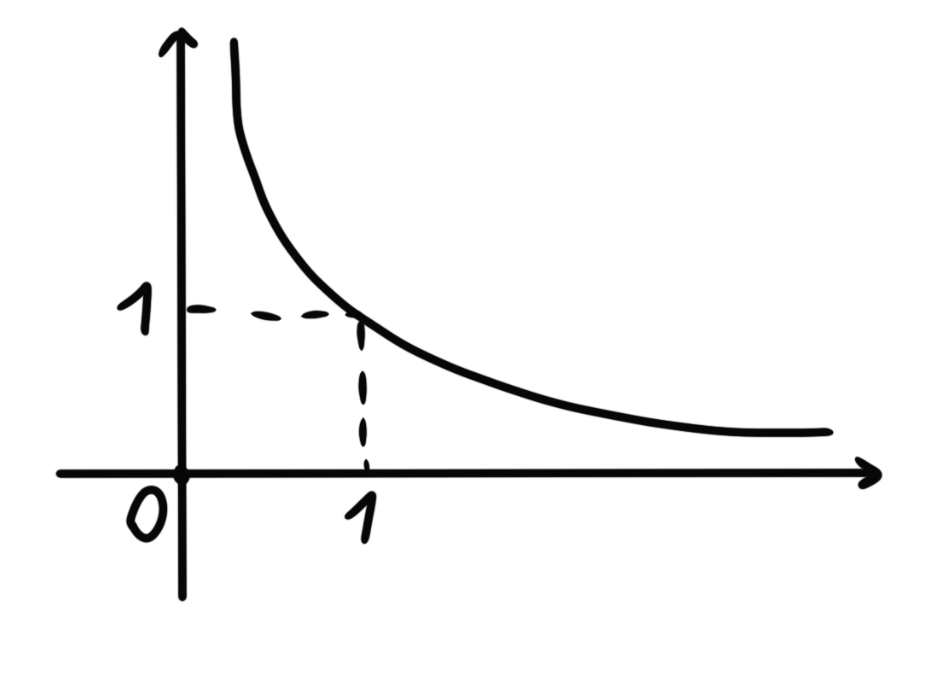
\includegraphics[width=0.5\textwidth]{/Users/vladbelousov/Desktop/Semestr_4-FP-NSU/ДфУ/Лекции_по_дням/image/29.png}
\end{center}

\[ f  \in  C (B ) , \text{ } \exists  \frac{\partial  f }{\partial y  }  \in  C (B ) , \text{ }  \exists  \frac{\partial  f }{\partial  \mu} \in  C ( \mathbb{R} ) , \text{ }  (1, 1, 0 ) \in \mathbb{R} ^3 \] 

Возьмем  \( [ t_1, t_2 ] \subset (  0, + \infty  ) \) 

\[ \Rightarrow 0 ) \exists  \Delta > 0 :  \forall \mu    : |\mu| < \Delta \Rightarrow y(t, \mu ) \text{ - определено на } [t_1,t_2 ]   \] 

\[ \Rightarrow 1) \exists  \frac{\partial  y }{\partial  \mu } ( t, \mu ) \in  C ( P )  \] 

\[ \Rightarrow y(t, \mu ) = \underbrace{y ( t, 0 )}_{\frac{1}{t  } } + \frac{\partial  y } {\partial  \mu } (t ,0 ) \mu    + o( \mu ) , \text{ } t \in  [t_1,t_2 ]  \] 

\[ \begin{cases}
    \frac{\partial  }{\partial  t } y ( t, \mu ) = 4 t \mu - y ^2 ( t, \mu )  \\
    y ( t ,\mu)  |_{t =1 }  =1 
\end{cases} \] 

Дифференцируем по \( \mu  \): 

\[ \begin{cases}
    \displaystyle \frac{\partial  }{\partial  \mu } \frac{\partial  }{\partial  t } y(t ,\mu ) = 4 t - 2 y(t,\mu)   \cdot \frac{\partial  y }{\partial  \mu }(t,\mu ) \\
    \displaystyle \frac{\partial  }{\partial  \mu } y (t,\mu ) |_{t =1 }  =0 
\end{cases} \] 

\[ \begin{cases}
\displaystyle \frac{\partial  }{\partial  t } \underbrace{\frac{\partial  y }{\partial  \mu } (t ,\mu )}_{ v(t, \mu)} = 4 t - 2 y ( t, \mu ) \cdot \underbrace{\frac{\partial  y }{\partial  \mu } (t ,\mu )}_{ v(t, \mu)}   \\
\displaystyle \underbrace{\frac{\partial  y }{\partial  \mu } (t ,\mu )}_{ v(t, \mu)}|_{t =1 }  =0 
\end{cases} \] 

\[ \mu = 0 : \text{ Обозначим } w (t ) = \frac{\partial  y } {\partial  \mu } (t , \mu ) |_{\mu =0}    \] 

\[\begin{aligned}
    \begin{cases}
        \displaystyle \frac{\partial  }{\partial  t }w (t ) = 4 t - 2 y (t, 0 ) w (t ) \\ 
        w(t ) |_{t =1} = 0  
    \end{cases}
    \begin{cases}
    \displaystyle w' = 4 t - \frac{2}{t }  w \\ 
    w(1 ) = 0
    \end{cases}
\end{aligned} \] 

1) Ищем решение однородного уравнения: 

\[ \displaystyle w ' = -\frac{2}{t } w \Rightarrow  w  =  \frac{c}{t ^2 }  \]

2) Ищем частное решение: 

\[ \displaystyle  w( t ) = \frac{ u (t )}{t ^2 }   \] 

\[ \frac{ u ' (t )}{t ^2 } - \frac{ 2 u(t )}{t ^3} = 4 t - \frac{2}{t }  \frac{u (t )}{t ^2 } \Rightarrow u'(t ) = 4 t ^3    \] 

\[ u(t ) = t ^4 + \tilde{c }\] 

3) Общее решение неоднородного уравнения: 

\[ w(t ) =  \frac{ t ^{ 4 }  + c }{t ^2 } = \frac{ t ^{ 4 } -1       }{ t ^2 }   \] 

\[ \Rightarrow y (t ,\mu ) = \frac{1}{t } + \frac{ t ^ 4 - 1 }{t ^2 } \mu + o(\mu ) , \text{ }  t \in  [t_1 ,t_2 ] \subset (0, + \infty  ) , \text{ }  |\mu     |< \Delta   \] 

\[ \begin{aligned}
    \begin{cases}
        y ' = f(t, y ) \\ 
        y(t_0 )= y_0 
        \end{cases} 
        \quad \Rightarrow \quad  y (t, y_0 )
\end{aligned} \] 

\[ f: \mathbb{D} \to  \mathbb{R} , \text{ }  \mathbb{D} \subset \mathbb{R} ^2 , \text{ }  \mathbb{D} \text{  - непустое открытое множество}  \] 

\begin{theorem}(Теорема 4.)
    Пусть \( f \in  C (\mathbb{D} ) , \text{ } \exists \frac{\partial  f }{\partial  y } \in  C(\mathbb{D} )   \). Пусть \( (t_0 , y_0 ^* ) \in  \mathbb{D} , \text{  } y(t ,y_0^* ) \) определено на \( (\alpha , \omega ) \). Возьмем \( [t_1,t_2 ] \subset (\alpha \omega ) \). Тогда: 
    
    0) \( \exists  \Delta > 0 , \text{ } \forall  y_0 : |y_0 - y_0 ^* | < \Delta \Rightarrow y(t, y_0 )  \)  определено на \( (\alpha , \omega) \) 

    1) \( \exists \frac{\partial  y }{\partial  y_0 } \in  C (P )  \), где \( P = \{(t, y_0 ): t \in  [t_1 ,t_2 ] , \text{ } |y_0 - y_0 ^* < \Delta|\} \)  

    2) \( \exists  \frac{\partial  ^2 y }{\partial  \mu \partial  t }  = \frac{\partial  ^2 y }{\partial  y_0 \partial  t_0 } \in C(P) \) 

    3) \( v(t, y_0 ) = \frac{\partial  y }{\partial  y_0 } (t,y_0 )   \)  -решение задачи Коши \( \begin{cases}
    \displaystyle \frac{\partial  }{\partial  t }v = \frac{\partial  f }{\partial  y } v  \\ 
    v (t_0 ) =1   
    \end{cases} \) 
\end{theorem}





%%-------------------------------%%

% Закрытие документа, если файл компилируется отдельно
\ifdefined\mainfile
    % Если это основной файл, не нужно заканчивать документ
\else
    \end{document}
\fi